% vim: set filetype=tex spell :

\chapter{Verification}

\label{ch:Verification}

The \ac{ACDS} consists of experimental hardware controlled by experimental software and as such requires a significant amount of verification to make sure everything functions on orbit. Ideally everything would be verified before launch but, it is difficult to replicate the on-orbit environment closely. The magnetic field can be effectively simulated using the Helmholtz cage so the sensors can be calibrated and tested. 

\section{Magnetometer Verification}

There are several steps to the magnetometer on a \ac{SPB} calibrated and verified. First the board is tested separate from the rest of the CubeSat. Next the \ac{SPB} is attached to the CubeSat and the torquer compensation routine is run to calculate the torquer offsets. Finally the compensation values are transfered to the \ac{ACDS} board and the compensation is verified.

\subsection{Initial Verification}

The magnetometer verification is done using the Helmholtz cage. A calibration is run on a board separate from the CubeSat. The calculations are done on the calibration coefficients so that they can be compared to the datasheet values to check if the magnetometers are preforming as they should. Problems are often caused by bad solder joints which can cause one or more axis to be unresponsive.

\begin{comment}
\subsection{Torquer offsets}

\begin{figure}[!ht]
    \centering
    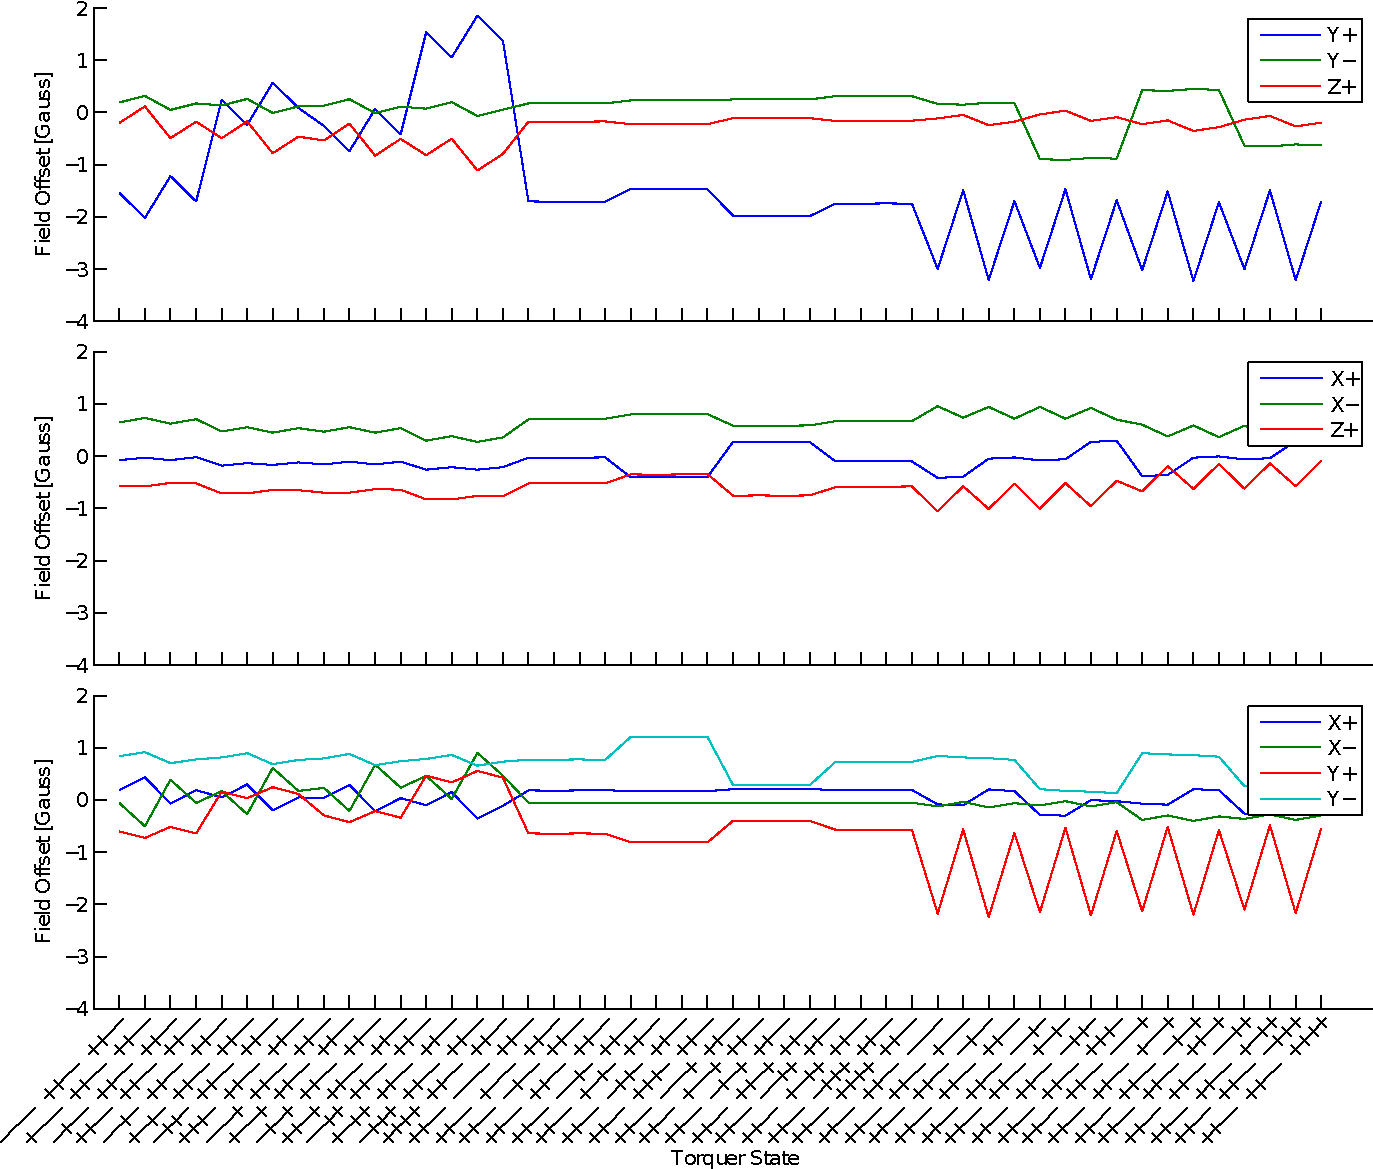
\includegraphics[width=0.8\linewidth]{board-offsets}
    \caption{Board offsets}
    \label{fig:b-offset}
\end{figure}

Because of the nature of the dipole magnetic field, the offsets measured by each magnetometer are unique to each magnetometer and torquer combination. Some torquers have only a small effect on each magnetometer and some have a much larger effect. \Cref{fig:b-offset} shows the offsets when the torquers are stepped through all possible states. The offsets are calculated for each board by sweeping the Helmholtz cage through a field pattern in the plane of each board. The offsets are rotated from the \ac{SPB} frame into the satellite frame and plotted on the same axis for comparison.

In \Cref{fig:b-offset} the largest offset appears to be both of the Y-axis torquers and one of the X-axis torquers cting on the X-axis \ac{SPB} in the Z-axis. When all three torquers are biased in a positive direction the offset is around 1.5 Gauss. When all three torquers are biased in the negative direction the offset is around -1.7 gauss.

\end{comment}

\subsection{Compensation Testing}

\begin{figure}[!ht]
    \centering
    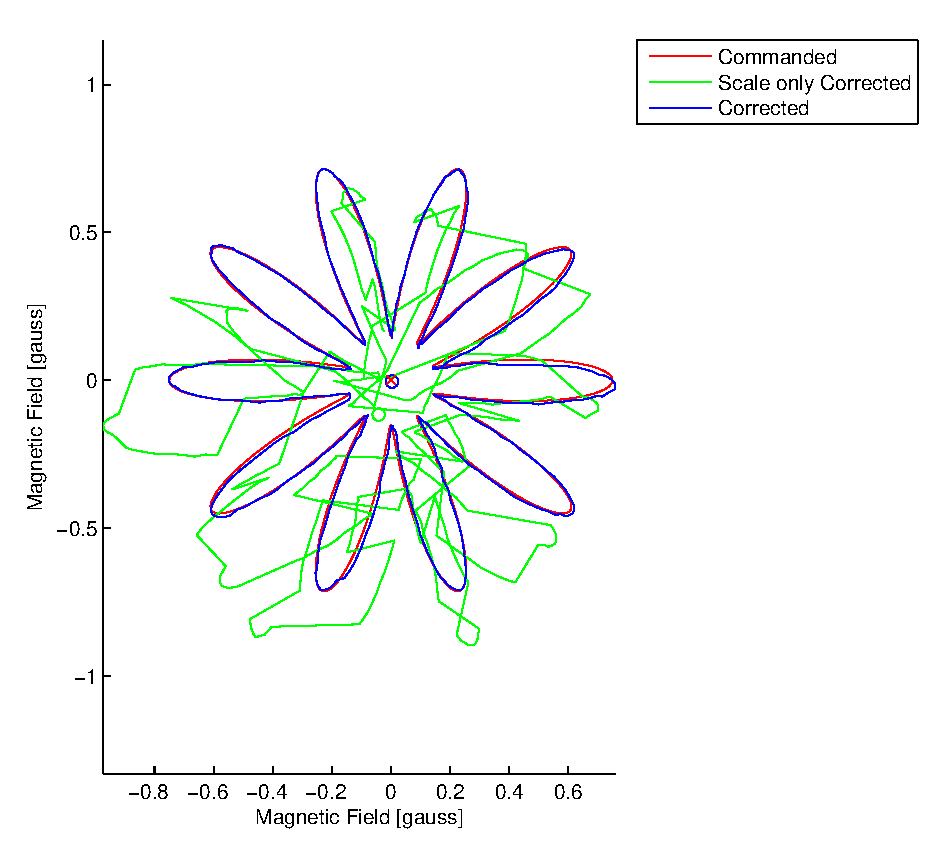
\includegraphics[width=0.8\linewidth]{torqueCalTst}
  \caption{A torquer compensation test showing that the correction provides a large amount of improvement over the uncorrected values}
    \label{fig:tqtst}
\end{figure}

The torquer compensation is tested using the tCalTstFull function. The function runs the Helmholtz Cage through a field sequence and takes measurements at each point. During the process a random torquer is flipped every 10 data points. The measurements are corrected, in Matlab, using the compensation data set and compared to the expected field. A typical plot of the data is shown in \cref{fig:tqtst}. The RMS error is also calculated for the data set so the effectiveness of the torquer compensation can be compared to the calibration without torquers.

\begin{lstlisting}[caption={Running torquer compensation test for the X+ \ac{SPB}},label={lst:tCalTst},language=Matlab]
a = [0 0 1;-1 0 0;0 1 0];
tCalTstFull('X+',cor,'COM3',57600,-95.3,1,a);
\end{lstlisting}

\Cref{lst:tCalTst} shows how to run the tCalTstFull function. The first argument to the tCalTstFull function is the address of the \ac{SPB} to use. The address can be specified as a number or, more continently, as a symbolic name that resolves to the correct address. The seccond argument is the correction that was previously calculated using the calall function. The third and fourth arguments are the serial port and buad rate to use to talk to the CubeSat. The fifth argument is the gain of the amplifier on the \ac{SPB} this is not really used for the calibration test because the gain is factored into the correction data. The 6th argument is the \ac{ADC} gain, this gain has already been factored into the calibration but it must be set correctly in the \ac{ADC} for the test to work properly. The last argument is the rotation matrix  The function needs a rotation matrix to transform from \ac{SPB} coordinates to Helmholtz cage coordinates. The code generates the magnetic field and plots the results in the \ac{SPB} plane.

\begin{figure}[!ht]
    \centering
    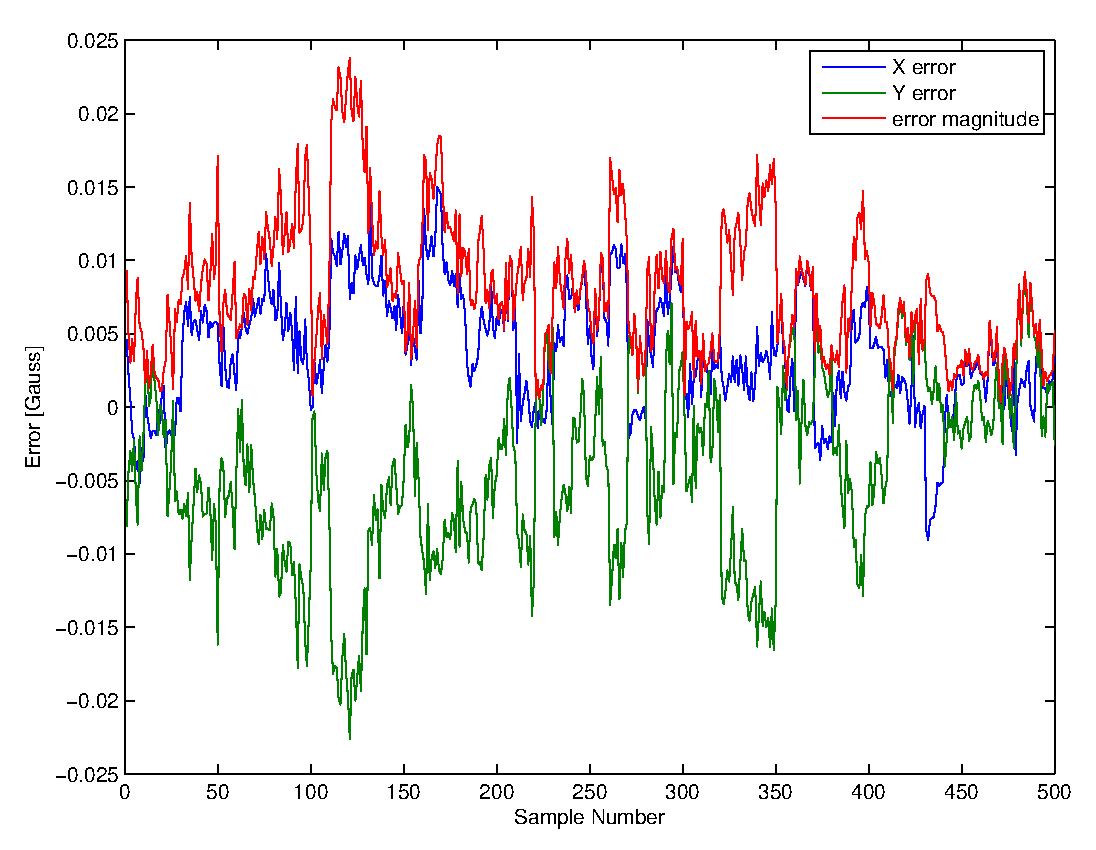
\includegraphics[width=0.8\linewidth]{torqueCalTst-err}
    \caption{Graph showing a torquer compensation error plot}
    \label{fig:tqerr}
\end{figure}

\Cref{fig:tqerr} shows the error for the torquer compensation test. The RMS error for the compensated data is 9 mGauss. The maximum error is 24 mGauss. On a 300 mGauss field a 24 mGauss error will cause an angular error of \textpm5\textdegree. The addition of the torquers causes an increase in the RMS and maximum error.
%This can be seen by comparing \cref{fig:tqerr} with \cref{fig:magerr}. In \cref{fig:tqerr} steps in the error are seen as torquers are flipped whereas in \cref{fig:magerr} the error is more consistent across the entire run.


\subsubsection{Embedded Compensation Testing}

The test in \cref{fig:tqtst,fig:tqerr} only used the \ac{ACDS} embedded system to flip torquers and take measurements. To Matlab was used to do all of the calculations for the calibration. During the flight the calibration must be done on-board with the embedded system on the \ac{ACDS} board.

\begin{figure}[!ht]
    \centering
    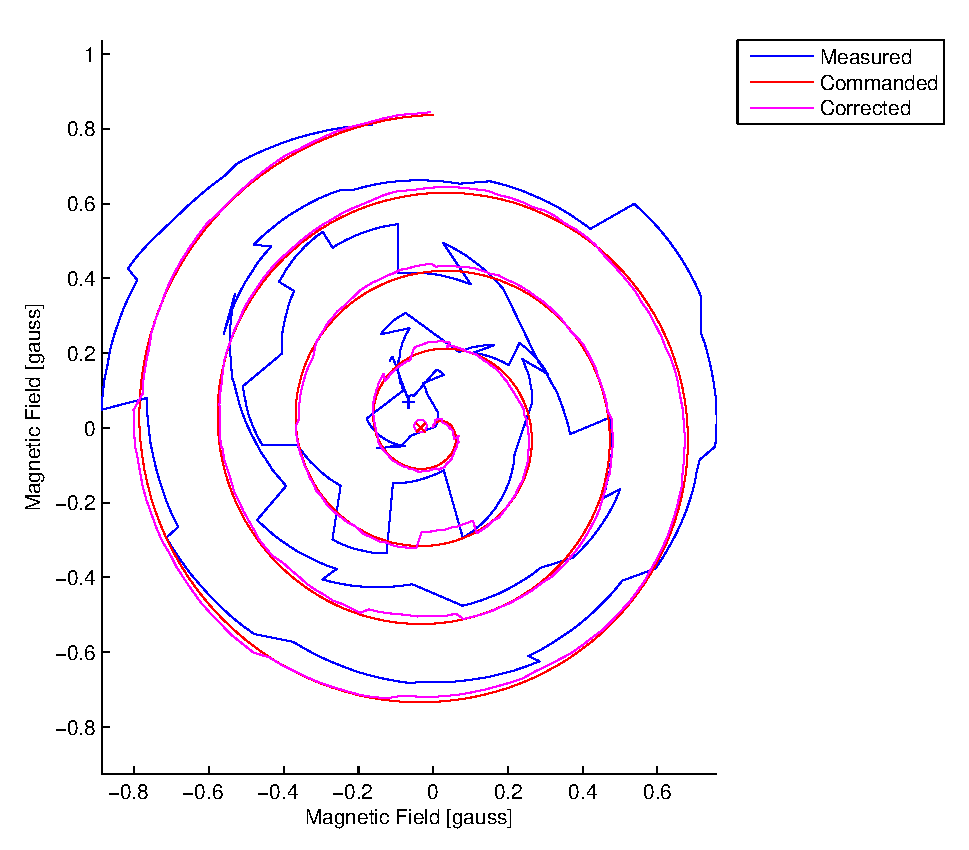
\includegraphics[width=1\linewidth]{torqueCalTstMSP}
    \caption{Test of the calibration as performed by the \ac{ACDS} board}
    \label{fig:tcalMSP}
\end{figure}

\Cref{fig:tcalMSP} shows the torquer calibration test using the Y+, Y- and Z+ \acp{SPB} with the calibration performed using the embedded system on the \ac{ACDS} board. The RMS error was 14.637793~mGauss. The maximum error was 39.054539~mGauss.

\begin{figure}[!ht]
    \centering
    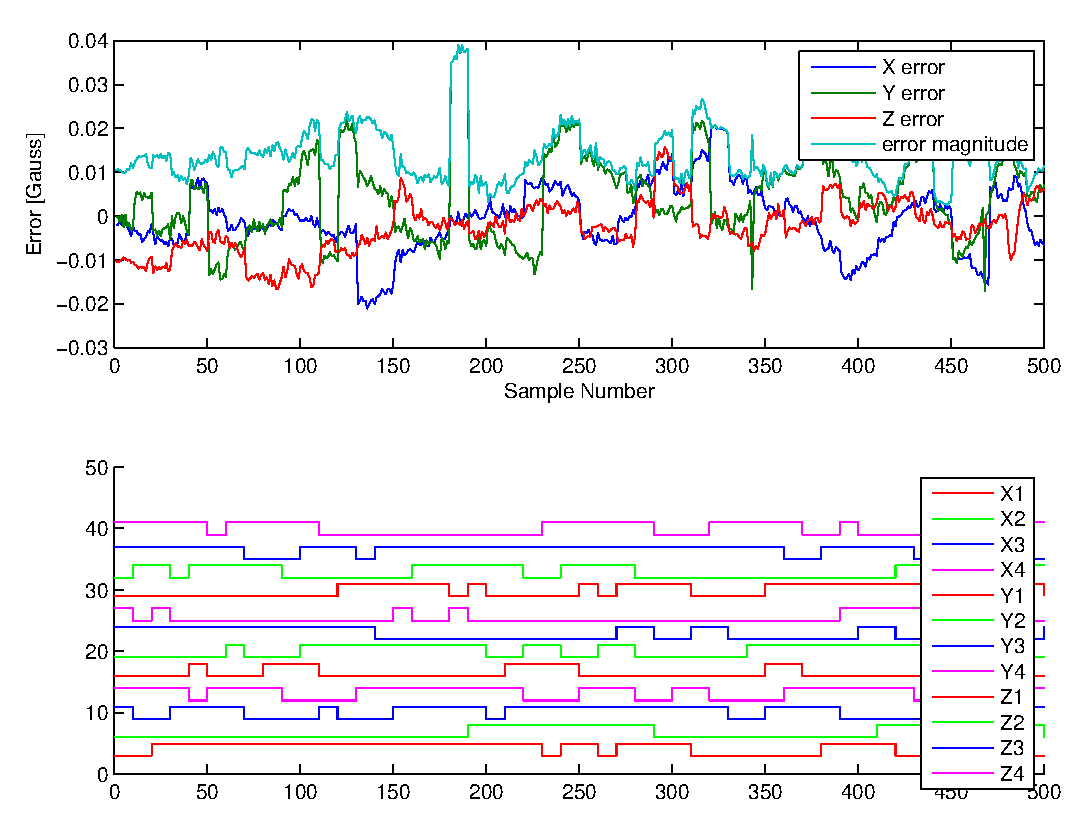
\includegraphics[width=1\linewidth]{torqueCalTstMSP-err-flips}
    \caption{Error plot for \cref{fig:tcalMSP} showing torquer states}
    \label{fig:tcalMSPerr}
\end{figure}

\Cref{fig:tcalMSPerr} shows the errors for each sample as well as the torquer states during the samples. The large jumps in the errors all correspond with torquer flips.

\begin{figure}[!ht]
    \centering
    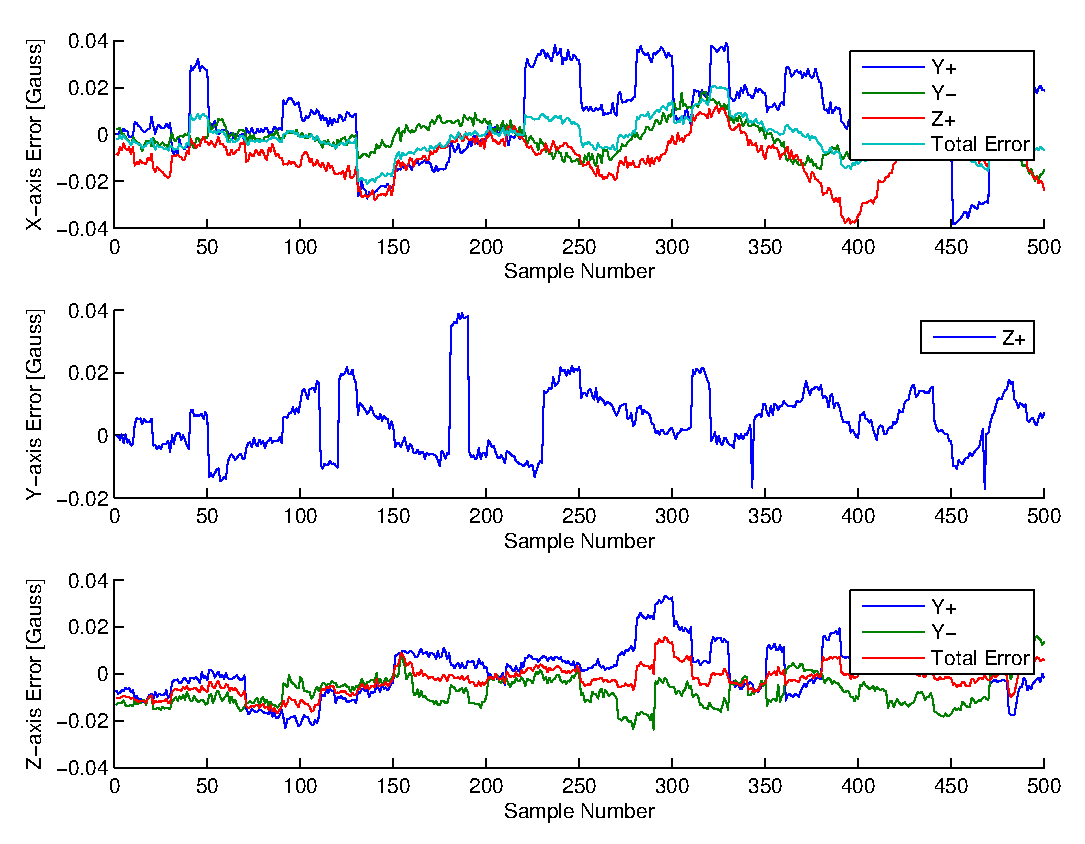
\includegraphics[width=1\linewidth]{torqueCalTstMSP-err-axes}
    \caption{Plot of magnetic field errors for each axis}
    \label{fig:tcalMSPerr-axis}
\end{figure}

\Cref{fig:tcalMSPerr-axis} shows the errors from each board in each axis. \Cref{tab:tcalMSPerr} shows the RMS errors in table form.

\begin{table}[!ht]
    \centering
    \caption{Errors for \ac{ACDS} system calibration test}
    \label{tab:tcalMSPerr}
    \begin{tabular}{|c|c|c|c|}
        \hline
        &X-axis&Y-axis&Z-axis\\
        \hline
        Y+&0.018473&N/A&0.011453\\
        \hline
        Y-&0.007671&N/A&0.009875\\
        \hline
        Z+&0.013049&0.010704&N/A\\
        \hline
        Total&0.007594&0.010704&0.006483\\
        \hline
    \end{tabular}
\end{table}

\begin{comment}
X-axis errors:
    Y+ RMS error = 0.018473
    Y- RMS error = 0.007671
    Z+ RMS error = 0.013049
Total X-axis error = 0.007594

Y-axis errors:
    Z+ RMS error = 0.010704
Total Y-axis error = 0.010704

Z-axis errors:
    Y+ RMS error = 0.011453
    Y- RMS error = 0.009875
Total Z-axis error = 0.006483
\end{comment}

\clearpage
\subsubsection{Torquer Repeatability}

The torquer compensation method depends on the torquer offsets being repeatable. If the offsets are not very repeatable then the offsets will induce errors in the measured field. \Cref{fig:tqoff} shows a plot of the torquer offsets. The plot shows the offsets of the torquers when they are polarized in each direction. The offset for both of the magnetometer axes are shown. To create the plot each torquer was flipped 20 times in each direction. After each flip a magnetometer calibration was done to get the offset values. The offset values are normalized to show deviation from the median for better comparison. The maximum offset variation in \cref{fig:tqoff} is 20 mGauss.

\begin{figure}[!ht]
    \centering
    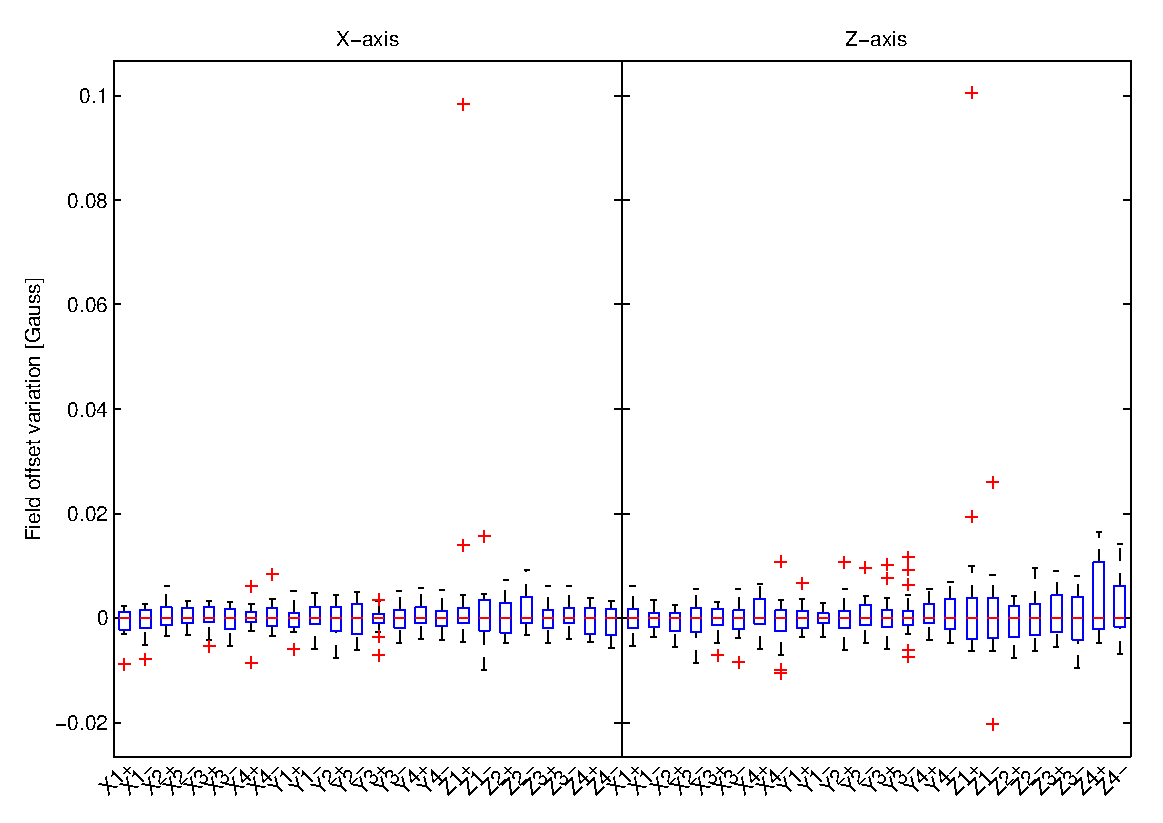
\includegraphics[width=0.9\linewidth]{torqueOffsets}
    \caption{Box Plot from torquer offset test}
    \label{fig:tqoff}
\end{figure}

The offset variations shown in \cref{fig:tqoff} are all less than the maximum error from \cref{fig:tqerr}. This is likely because the maximum offsets did not occur all at the same time.

\section{B-dot controller simulations}

To verify the B-dot algorithm the \ac{ACDS} is placed in the helmholtz cage and a rotating field is generated. The minimum rotation rate of the magnetic field that will cause a rotation rate is calculated by starting with \cref{eq:bdot-cross}

\begin{equation}
    \dot{\vec{B}} = \vec{B} \cross \omega
    \label{eq:bdot-cross}
\end{equation}

If the axis of rotation is perpendicular to the field rotation then \cref{eq:bdot-cross} becomes \cref{eq:bdot-mul}

\begin{equation}
    \dot{\vec{B}} = \left| \vec{B} \right| \cdot \left| \omega \right|
    \label{eq:bdot-mul}
\end{equation}

The B-dot algorithm equation is shown in \cref{eq:bdot-alg}.

\begin{equation}
    M_{cmd} = C \dot{\vec{B}} 
    \label{eq:bdot-alg}
\end{equation}

Substituting \cref{eq:bdot-mul} into \cref{eq:bdot-alg} and solving for $\omega$ gives \cref{eq:omega-th}. Where $M_{th}$ is the torque switching threshold for the torquers and $\omega_{th}$ is the minimum rotation rate required to flip a torquer.

\begin{equation}
    \omega _ {th} = {M _ {th} \over{ {C \left| \vec{B} \right|}}}
    \label{eq:omega-th}
\end{equation}

If a 0.5 gauss field is used and $C$ is 200 and the torquer switching threshold is $0.022 \unit{A \cdot m} ^2$ then $\omega_{th}$ is calculated as follows

\begin{equation}
    \omega _ {th} = { 0.022 \over{ {200 \cdot 0.5}}} = 0.00022 ~ \unit{rad / sec}
\end{equation}

\begin{figure}[!ht]
    \centering
    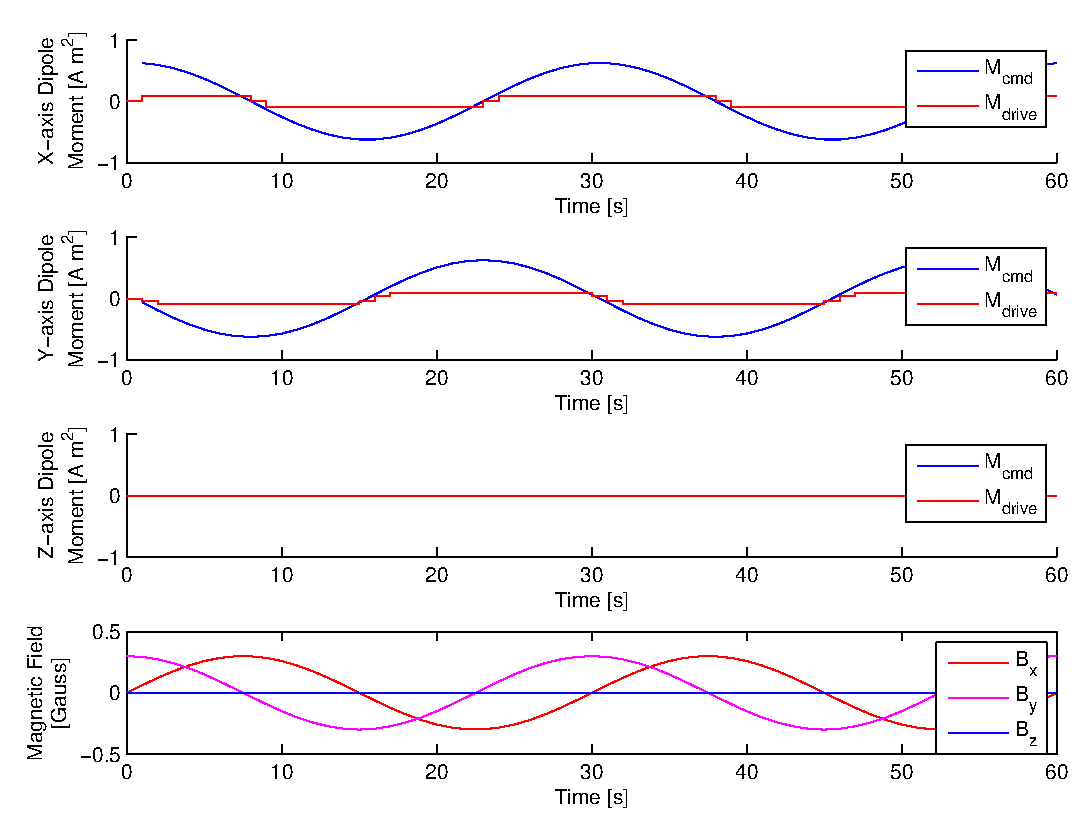
\includegraphics[width=1\linewidth]{detumble-sim}
  \caption{Simulation of torquer output with spinning magnetic field}
    \label{fig:detumble-sim}
\end{figure}

%With the field set to $\omega_{th}$ a torquer should flip as $\dot{\vec{B}}$ becomes aligned with a torquer axis as the field continues to sweep the torquer will switch off.

\Cref{fig:detumble-sim} shows a simulation of the detumble algorithm in a spinning magnetic field. The field has a magnitude of 0.3~Gauss spins around the Z-axis. The plots show the magnetic dipole moment that the algorithm wants to drive and is able to drive as the magnetic field spins around.


\section{Detumble Flip Test}

\Cref{fig:detumble-test} shows the results of the detumble test. This is the same as the detumble simulation in \cref{fig:detumble-sim} except the field has been programed into the Helmholtz cage, measured by the \acp{SPB}, calculations done by the \ac{ACDS} and torquers flipped in an attempt to stop the motion.

\begin{figure}[!ht]
    \centering
    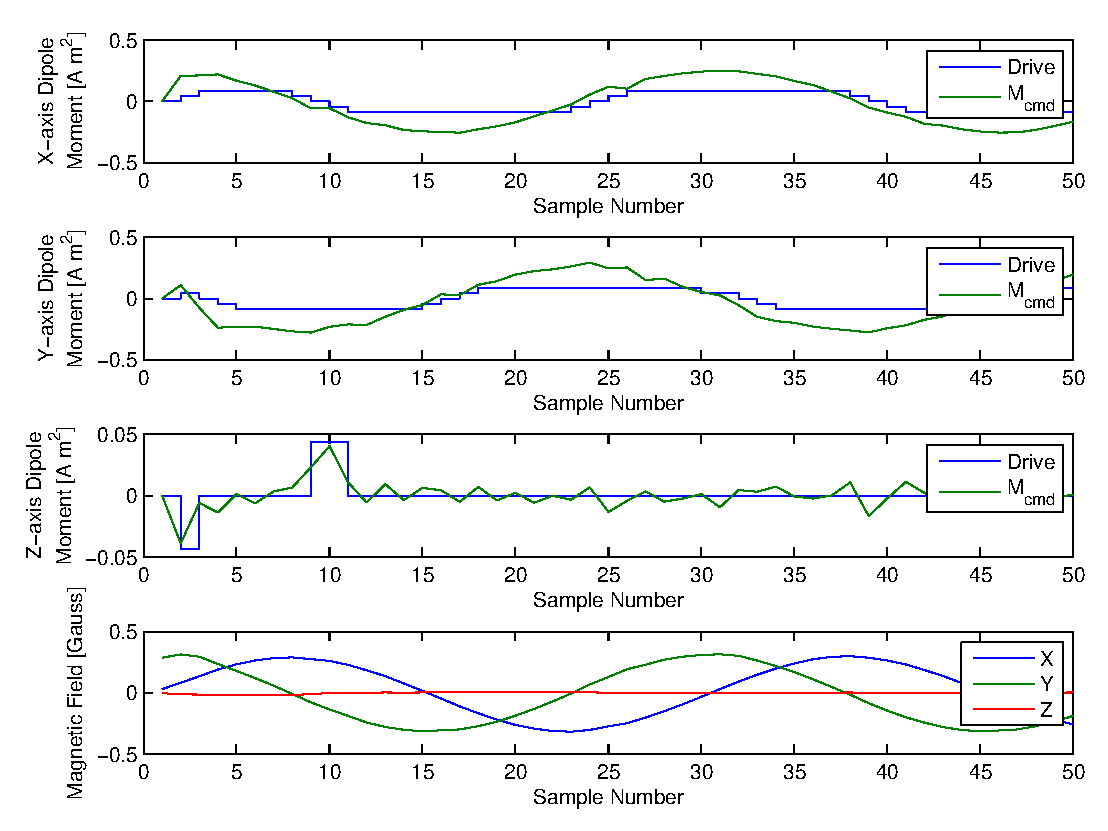
\includegraphics[width=1\linewidth]{detumble-test}
  \caption{Test of the B-dot controller}
    \label{fig:detumble-test}
\end{figure}

The results in \cref{fig:detumble-test} are similar to the results in the simulation in \cref{fig:detumble-sim}. The main difference is that there are some unexpected flips in the Z-axis. This is due to noise in the magnetic field causing torquers to be flipped. It is unclear if the noise is caused by the enviornment in the Helmholtz cage or by torquer flips and imperfect torquer calibration.


